\documentclass[12pt, a4paper]{article}

% ── Packages ──────────────────────────────────────────────────────────
\usepackage[margin=1in]{geometry}
\usepackage{graphicx}
\usepackage{amsmath, amssymb}
\usepackage{booktabs}
\usepackage{hyperref}
\usepackage{xcolor}
\usepackage{listings}
\usepackage{enumitem}
\usepackage{caption}
\usepackage{subcaption}
\usepackage{float}
\usepackage{titlesec}
\usepackage{fancyhdr}
\usepackage{abstract}
\usepackage{microtype}
\usepackage{setspace}
\usepackage{parskip}
\usepackage{tikz}
\usetikzlibrary{shapes.geometric, arrows.meta, positioning, fit, backgrounds}

% ── Colours ───────────────────────────────────────────────────────────
\definecolor{primary}{RGB}{44, 90, 160}
\definecolor{accent}{RGB}{0, 180, 160}
\definecolor{lightgray}{RGB}{245, 245, 245}
\definecolor{codegray}{RGB}{100, 100, 100}
\definecolor{codegreen}{RGB}{40, 130, 60}
\definecolor{codepurple}{RGB}{140, 40, 160}

% ── Hyperref setup ────────────────────────────────────────────────────
\hypersetup{
    colorlinks=true,
    linkcolor=primary,
    urlcolor=accent,
    citecolor=primary,
    pdftitle={House Price Prediction and Agentic AI Real Estate Advisory},
    pdfauthor={Vedant Madne},
}

% ── Code listing style ────────────────────────────────────────────────
\lstdefinestyle{codestyle}{
    backgroundcolor=\color{lightgray},
    commentstyle=\color{codegreen}\itshape,
    keywordstyle=\color{primary}\bfseries,
    stringstyle=\color{codepurple},
    basicstyle=\ttfamily\small,
    breakatwhitespace=false,
    breaklines=true,
    captionpos=b,
    keepspaces=true,
    numberstyle=\tiny\color{codegray},
    numbers=left,
    numbersep=6pt,
    showspaces=false,
    showstringspaces=false,
    tabsize=4,
    frame=single,
    rulecolor=\color{gray!30},
    xleftmargin=12pt,
}
\lstset{style=codestyle}

% ── Section formatting ────────────────────────────────────────────────
\titleformat{\section}
  {\large\bfseries\color{primary}}
  {\thesection.}{0.6em}{}[\vspace{-0.3em}\rule{\linewidth}{0.6pt}]

\titleformat{\subsection}
  {\normalsize\bfseries\color{primary!80!black}}
  {\thesubsection.}{0.5em}{}

\titleformat{\subsubsection}
  {\normalsize\bfseries}
  {\thesubsubsection.}{0.5em}{}

% ── Header / Footer ───────────────────────────────────────────────────
\pagestyle{fancy}
\fancyhf{}
\fancyhead[L]{\small\textcolor{gray}{House Price Predictor \& AI Advisory System}}
\fancyhead[R]{\small\textcolor{gray}{End-Semester Report}}
\fancyfoot[C]{\thepage}
\renewcommand{\headrulewidth}{0.4pt}

\setlength{\parskip}{6pt}
\onehalfspacing

% ══════════════════════════════════════════════════════════════════════
\begin{document}

% ── Title Page ────────────────────────────────────────────────────────
\begin{titlepage}
  \centering
  \vspace*{1.5cm}

  {\fontsize{22}{28}\selectfont\bfseries\color{primary}
    House Price Prediction and\\[0.4em]
    Agentic AI Real Estate Advisory System
  }

  \vspace{0.8cm}
  \rule{0.6\linewidth}{1.2pt}
  \vspace{0.8cm}

  {\large\color{gray} End-Semester Project Report --- Milestone 2}

  \vspace{1.5cm}

  {\large \textbf{Vedant Madne}}\\[0.3em]
  {\normalsize nst.b2b.marketing@gmail.com}

  \vspace{2.5cm}

  \begin{tabular}{ll}
    \textbf{Dataset}    & King County, Washington --- House Sales (2014--2015) \\[4pt]
    \textbf{Stack}      & Python · Streamlit · LangGraph · RAG · HuggingFace LLM \\[4pt]
    \textbf{Deployment} & Streamlit Cloud \\[4pt]
    \textbf{Repository} & \url{https://github.com/vedant-valid/house-price-prediction-ml} \\
  \end{tabular}

  \vfill
  {\small \today}
\end{titlepage}

% ── Abstract ──────────────────────────────────────────────────────────
\begin{abstract}
\noindent
This report documents the design, implementation, and evaluation of a two-phase
real estate intelligence system built for King County, Washington. The first phase
applies classical supervised machine learning --- Linear Regression, Random Forest,
and XGBoost --- to predict residential sale prices from 18 property features across
4,600 transactions. After log-transforming the target and applying standard
preprocessing, Linear Regression achieved the best generalisation
($R^2 = 0.80$, $\text{MAE} = \$81{,}492$), confirming that log-price in this dataset
is largely additive.

The second phase extends the predictor into a full \textit{agentic AI advisory assistant}.
Using LangGraph for multi-step workflow orchestration, a TF-IDF retrieval module for
Retrieval-Augmented Generation (RAG) over a curated market knowledge base, and a
large language model (Qwen-2.5-72B) for structured report generation, the system
autonomously analyses a property, retrieves relevant market trends, finds comparable
sales, and produces a grounded BUY / HOLD / AVOID investment recommendation. Responsible
AI practices --- including RAG grounding to prevent hallucination and a mandatory
disclaimer --- are embedded throughout the pipeline.
\end{abstract}

\tableofcontents
\newpage

% ══════════════════════════════════════════════════════════════════════
\section{Introduction}
% ══════════════════════════════════════════════════════════════════════

Residential real estate is one of the most significant financial decisions most
people make in their lifetime, yet price discovery remains opaque and highly dependent
on local expertise. A buyer evaluating a three-bedroom house in Bellevue, Washington
must simultaneously reason about square footage norms, neighbourhood price tiers,
market seasonality, property condition, and comparable recent sales --- a task that
typically requires a licensed agent with years of local experience.

This project addresses that gap in two stages. \textbf{Milestone 1} builds a
machine learning model that takes structured property attributes as input and
outputs a predicted sale price with a confidence range. \textbf{Milestone 2} wraps
that predictor inside an \textit{agentic} AI system: one that does not merely return
a number, but reasons step by step --- retrieving market context, identifying
comparable homes, and generating a plain-language investment advisory report grounded
in real data.

The goals of this project are:
\begin{itemize}[leftmargin=1.4em]
  \item Train and evaluate multiple regression models on King County house sales data.
  \item Deploy an interactive web application for real-time price estimation.
  \item Design an agentic multi-step pipeline using LangGraph with explicit state management.
  \item Integrate RAG to ground LLM outputs in curated market knowledge.
  \item Surface actionable, responsible AI-driven investment recommendations.
\end{itemize}

% ══════════════════════════════════════════════════════════════════════
\section{Dataset and Problem Formulation}
% ══════════════════════════════════════════════════════════════════════

\subsection{Dataset Overview}

The dataset contains \textbf{4,600 residential property sales} in King County,
Washington recorded between 2014 and 2015. Each record describes a single
transaction with 18 raw columns spanning structural, locational, and quality
attributes.

\begin{table}[H]
\centering
\caption{Key dataset statistics}
\begin{tabular}{ll}
  \toprule
  \textbf{Attribute}        & \textbf{Value} \\
  \midrule
  Total transactions        & 4,600 \\
  Unique cities             & 44 \\
  Unique ZIP codes          & 70+ \\
  Price --- mean            & \$551,963 \\
  Price --- median          & \$460,943 \\
  Price --- range           & \$0 -- \$26,590,000 \\
  Year built --- range      & 1900 -- 2014 \\
  Waterfront properties     & 33 (0.7\%) \\
  Condition (mode)          & 3 --- Average (2,875 homes) \\
  \bottomrule
\end{tabular}
\end{table}

The raw features include: \texttt{sqft\_living}, \texttt{sqft\_lot},
\texttt{sqft\_above}, \texttt{sqft\_basement}, \texttt{bedrooms},
\texttt{bathrooms}, \texttt{floors}, \texttt{waterfront}, \texttt{view},
\texttt{condition}, \texttt{yr\_built}, \texttt{yr\_renovated}, \texttt{city},
\texttt{statezip}, \texttt{date}, \texttt{street}, and \texttt{country}.

\subsection{Problem Formulation}

This is a \textbf{supervised regression} task. Given a feature vector
$\mathbf{x} \in \mathbb{R}^d$ describing a property, the objective is to learn a
function $f: \mathbb{R}^d \rightarrow \mathbb{R}$ such that:

\[
  \hat{y} = f(\mathbf{x}), \quad \text{where } \hat{y} \approx \log(1 + y_{\text{price}})
\]

The log-transform is applied because raw house prices are right-skewed (the $\$26.6M$
maximum inflates errors for ordinary homes). Predicting in log-space gives each price
tier equal weight and produces percentage-style errors that are more interpretable for
investors.

% ══════════════════════════════════════════════════════════════════════
\section{Milestone 1 --- Machine Learning Pipeline}
% ══════════════════════════════════════════════════════════════════════

\subsection{Data Preprocessing}

Raw data is processed through a deterministic pipeline (\texttt{preprocessing.py})
before any model sees it. The steps are:

\begin{enumerate}[leftmargin=1.6em]
  \item \textbf{Date parsing}: Extract \texttt{year\_sold} and \texttt{month\_sold}
        from the raw date string; drop the original \texttt{date} column.
  \item \textbf{Column pruning}: Remove identifiers (\texttt{street}, \texttt{country})
        that carry no generalisable signal.
  \item \textbf{Handling zero prices}: Rows with \texttt{price = 0} are removed as
        they represent data entry errors.
  \item \textbf{Log transformation}: Apply $y' = \log(1 + \text{price})$ to the
        target variable to normalise the distribution.
  \item \textbf{One-hot encoding}: Encode \texttt{city} and \texttt{statezip}
        categorically. With 44 cities and 70+ ZIP codes, this expands the feature
        space substantially but captures the dominant locational signal.
  \item \textbf{Standard scaling}: All numerical features are scaled using
        \texttt{StandardScaler} (zero mean, unit variance) to prevent features with
        large magnitudes from dominating distance-based components.
  \item \textbf{Train/test split}: 80\% training, 20\% test, random state fixed for
        reproducibility.
\end{enumerate}

\subsection{Models}

Three regression algorithms were trained and evaluated:

\subsubsection{Linear Regression}
Assumes price in log-space is a linear combination of features:
\[
  \hat{y}' = \mathbf{w}^\top \mathbf{x} + b
\]
After the log-transform and one-hot encoding, the feature-to-target relationship
is largely linear, which is why this model performs best on this specific dataset.

\subsubsection{Random Forest Regressor}
An ensemble of 100 decision trees trained on bootstrap samples. Each tree splits
on a random subset of features at each node. The final prediction is the mean of
all tree outputs:
\[
  \hat{y}' = \frac{1}{T} \sum_{t=1}^{T} h_t(\mathbf{x})
\]
Random Forest handles non-linear interactions well but tends to overfit when the
underlying relationship is genuinely linear.

\subsubsection{XGBoost}
A gradient-boosted tree ensemble that builds trees sequentially, each correcting
the residuals of the previous:
\[
  F_m(\mathbf{x}) = F_{m-1}(\mathbf{x}) + \eta \cdot h_m(\mathbf{x})
\]
where $\eta$ is the learning rate. XGBoost is powerful for tabular data with
complex feature interactions, but on this dataset the log-linear structure favours
simpler models.

\subsection{Model Evaluation}

Models were evaluated on the held-out test set and validated using 5-fold
cross-validation. All metrics are reported in the original price scale (inverse
log-transform applied to predictions).

\begin{table}[H]
\centering
\caption{Model performance comparison}
\begin{tabular}{lcccc}
  \toprule
  \textbf{Model}      & \textbf{R²}   & \textbf{CV R² (5-fold)} & \textbf{MAE}      & \textbf{RMSE}      \\
  \midrule
  Linear Regression   & \textbf{0.803} & \textbf{0.816}         & \textbf{\$81,492} & \textbf{\$138,943} \\
  XGBoost             & 0.788          & ---                     & ---               & ---                \\
  Random Forest       & 0.735          & ---                     & ---               & ---                \\
  Decision Tree       & 0.519          & ---                     & ---               & ---                \\
  \bottomrule
\end{tabular}
\end{table}

\textbf{Why does Linear Regression win?} The King County dataset, after
log-transformation and one-hot encoding, exhibits a near-linear relationship
between features and price. The dominant driver --- living area ($\texttt{sqft\_living}$)
--- has a log-linear relationship with price. Non-linear models add complexity without
capturing additional signal, and with only 4,600 samples, they risk overfitting.
The 5-fold CV $R^2 = 0.816$ confirms the linear model generalises stably.

The MAE of \$81,492 on a median property price of \$460,943 represents an
approximation error of approximately 17.7\% --- a practically useful bound for
an investor assessing whether an asking price is fair.

\subsection{Inference and Confidence Range}

At inference time (\texttt{inference.py}):
\begin{enumerate}[leftmargin=1.6em]
  \item The same preprocessing pipeline is applied to the input features.
  \item The saved scaler and model artifacts are loaded from \texttt{models/}.
  \item The model predicts in log-space; the output is inverse-transformed.
  \item A $\pm 10\%$ confidence band is applied to the predicted price to communicate
        model uncertainty to the user.
\end{enumerate}

% ══════════════════════════════════════════════════════════════════════
\section{Milestone 2 --- Agentic AI Advisory System}
% ══════════════════════════════════════════════════════════════════════

\subsection{Motivation and Design Philosophy}

A price estimate alone is not sufficient for an investor. To decide whether to buy,
hold, or avoid a property, one also needs to know: How does this price compare to
similar homes? What does the local market look like? Is this neighbourhood
appreciating or stagnating? Are there risks tied to the property's age or condition?

The Milestone 2 system answers all of these questions autonomously by decomposing
the advisory task into discrete, verifiable steps --- an \textit{agentic} approach
where each node in the pipeline has a single responsibility, and the system routes
between nodes based on the state accumulated so far.

\subsection{System Architecture}

\begin{figure}[H]
\centering
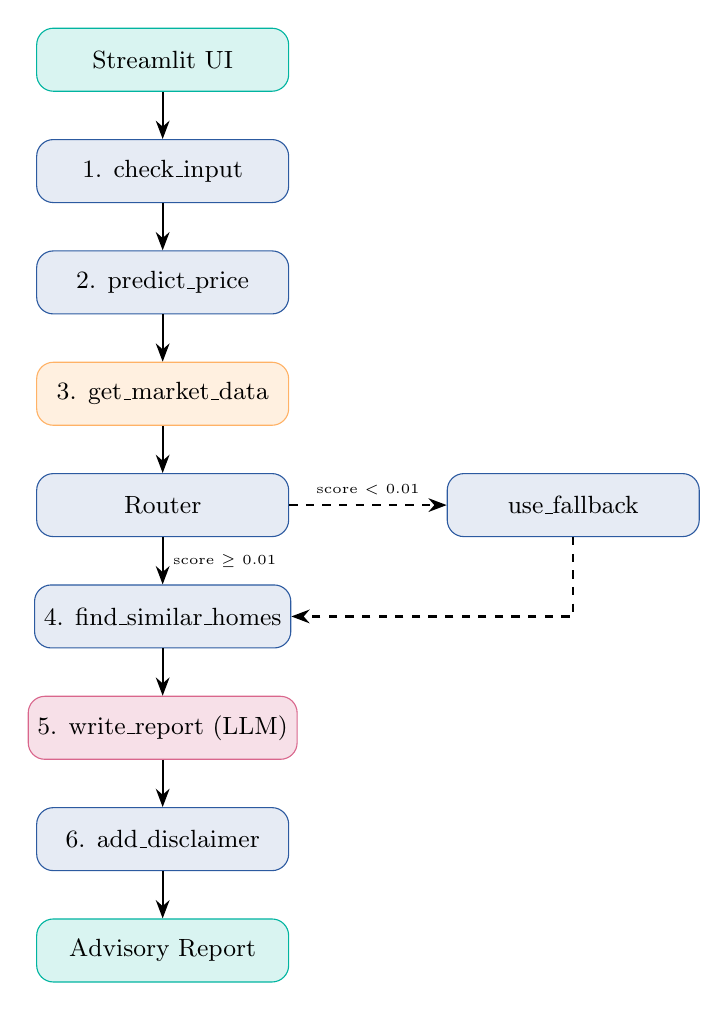
\begin{tikzpicture}[
    node distance=0.6cm and 1.2cm,
    box/.style={rectangle, rounded corners=6pt, minimum width=3.2cm,
                minimum height=0.8cm, text centered, draw, font=\small},
    userbox/.style={box, fill=accent!15, draw=accent},
    agentbox/.style={box, fill=primary!12, draw=primary},
    llmbox/.style={box, fill=purple!12, draw=purple!60},
    ragbox/.style={box, fill=orange!12, draw=orange!60},
    arrow/.style={-Stealth, thick},
    dasharrow/.style={-Stealth, thick, dashed},
]

\node[userbox] (ui)       {Streamlit UI};
\node[agentbox, below=of ui] (check)    {1. check\_input};
\node[agentbox, below=of check] (predict)  {2. predict\_price};
\node[ragbox,   below=of predict] (rag)     {3. get\_market\_data};
\node[agentbox, below=of rag] (router)   {Router};

\node[agentbox, right=2cm of router] (fallback) {use\_fallback};
\node[agentbox, below=of router] (comps)    {4. find\_similar\_homes};
\node[llmbox,   below=of comps] (report)   {5. write\_report (LLM)};
\node[agentbox, below=of report] (disc)     {6. add\_disclaimer};
\node[userbox,  below=of disc] (out)      {Advisory Report};

\draw[arrow] (ui)      -- (check);
\draw[arrow] (check)   -- (predict);
\draw[arrow] (predict) -- (rag);
\draw[arrow] (rag)     -- (router);
\draw[arrow] (router)  -- node[right, font=\tiny]{score $\geq$ 0.01} (comps);
\draw[dasharrow] (router) -- node[above, font=\tiny]{score $<$ 0.01} (fallback);
\draw[dasharrow] (fallback) |- (comps);
\draw[arrow] (comps)   -- (report);
\draw[arrow] (report)  -- (disc);
\draw[arrow] (disc)    -- (out);

\end{tikzpicture}
\caption{LangGraph agentic pipeline. Dashed arrows indicate the fallback path.}
\end{figure}

\subsection{LangGraph --- Workflow Orchestration}

LangGraph is a graph-based orchestration framework built on top of LangChain. It
represents the pipeline as a \textbf{directed state graph} where:
\begin{itemize}[leftmargin=1.4em]
  \item \textbf{Nodes} are Python functions, each responsible for one step.
  \item \textbf{Edges} define the flow between steps.
  \item \textbf{Conditional edges} allow runtime routing based on the accumulated state.
\end{itemize}

The key advantage of LangGraph over a simple sequential chain is that it makes
branching explicit and auditable. The router node inspects the retrieval confidence
score and chooses between the RAG-retrieved path and a safe fallback --- a design
choice that ensures the advisory report is never generated from empty context.

\subsection{Agent State}

All information flows through a single \texttt{AgentState} TypedDict that every
node reads from and writes to:

\begin{lstlisting}[language=Python, caption={AgentState definition (agent/state.py)}]
from typing import TypedDict, Optional

class AgentState(TypedDict):
    property_input:   dict         # raw user inputs
    predicted_price:  float        # output of ML model
    price_range:      dict         # {"low": ..., "high": ...}
    retrieved_docs:   list[str]    # top-k RAG chunks
    retrieval_score:  float        # cosine similarity score
    comparables:      list[dict]   # similar homes from data.csv
    report:           dict         # LLM-generated advisory
    error:            Optional[str]
\end{lstlisting}

Explicit state management means every intermediate result is inspectable.
If the pipeline fails at any step, the state contains enough context to diagnose
exactly where and why.

\subsection{Retrieval-Augmented Generation (RAG)}

\subsubsection{Why RAG?}
Large language models are prone to confabulating plausible-sounding but incorrect
statistics --- a particularly dangerous failure mode in a financial advisory context.
RAG mitigates this by retrieving factual snippets from a curated knowledge base and
injecting them into the LLM prompt as grounding context.

\subsubsection{Knowledge Base Construction}
The knowledge base consists of \textbf{10 plain-text files} generated from the
actual dataset by \texttt{rag\_builder.py}:

\begin{table}[H]
\centering
\caption{Market knowledge base files}
\begin{tabular}{ll}
  \toprule
  \textbf{File}                  & \textbf{Content} \\
  \midrule
  \texttt{zip\_price\_stats.txt}       & Median and mean price per ZIP code \\
  \texttt{city\_price\_stats.txt}      & Median price per city (44 cities) \\
  \texttt{feature\_impact.txt}         & Price by sqft band, bedrooms, condition \\
  \texttt{price\_tier\_analysis.txt}   & Q1, Q2, Q3, P90 price thresholds \\
  \texttt{neighborhood\_rankings.txt}  & Top 10 most/least expensive cities \\
  \texttt{market\_seasonality.txt}     & Price variation by month \\
  \texttt{waterfront\_premium.txt}     & Waterfront vs non-waterfront premium \\
  \texttt{king\_county\_overview.txt}  & General market context \\
  \texttt{investment\_principles.txt}  & General real estate investment rules \\
  \texttt{regulations\_disclaimer.txt} & Legal and regulatory context \\
  \bottomrule
\end{tabular}
\end{table}

\subsubsection{Retrieval Method}
Rather than using a heavy dense-embedding model, the retrieval layer uses
\textbf{TF-IDF} (Term Frequency--Inverse Document Frequency) with bigrams and
cosine similarity:

\[
  \text{TF-IDF}(t, d) = \text{tf}(t,d) \cdot \log\frac{N}{|\{d : t \in d\}|}
\]

\[
  \text{similarity}(q, d_i) = \frac{\mathbf{q} \cdot \mathbf{d}_i}{\|\mathbf{q}\|\,\|\mathbf{d}_i\|}
\]

The query is constructed from the user's property inputs (city, ZIP, sqft, bedroom
count) and matched against paragraph-level chunks from all knowledge files. The
top-4 most relevant chunks are retrieved and passed to the LLM. This approach
requires no model download, adds minimal latency, and performs well on the
keyword-rich real estate domain.

\subsection{LLM Report Generation}

\subsubsection{Model}
The advisory report is generated by \textbf{Qwen/Qwen2.5-72B-Instruct}, a 72-billion
parameter open-source instruction-tuned model served via the HuggingFace Inference API.

\subsubsection{Prompt Design and Hallucination Reduction}

The prompt is carefully structured to minimise hallucination:

\begin{enumerate}[leftmargin=1.6em]
  \item \textbf{Grounded context}: RAG-retrieved chunks and comparable sale prices
        are injected into the prompt. The model is explicitly instructed:
        \textit{"Do not invent statistics not present in the context."}
  \item \textbf{Explicit decision rules}: The prompt defines hard criteria for
        BUY, HOLD, and AVOID recommendations tied to measurable signals (condition
        score, price deviation from comparables, year built). This prevents the model
        from defaulting to optimistic recommendations.
  \item \textbf{Structured output}: The model is required to respond in a fixed JSON
        schema with three keys --- \texttt{summary}, \texttt{action}, \texttt{market\_notes}.
        Invalid or unparseable responses fall back gracefully.
  \item \textbf{Low temperature}: Temperature $= 0.3$ reduces creative variation in
        favour of factual consistency.
\end{enumerate}

\begin{lstlisting}[language={}, caption={Decision rules embedded in the advisory prompt}]
Decision Rules — follow these strictly:
- AVOID: condition <= 2, OR priced 10%+ above comparables,
         OR yr_built < 1960 with poor condition
- HOLD:  condition == 3 AND price within 5% of comparables,
         OR market context shows uncertain/slow demand
- BUY:   condition >= 4 AND price at or below comparable median,
         OR strong appreciation signals in market context
\end{lstlisting}

\subsubsection{Comparable Properties}
The \texttt{find\_similar\_homes} node searches \texttt{data.csv} directly for
properties matching $\pm 20\%$ of the input's living area, the same bedroom count,
and the same city where possible. The five closest matches by predicted price are
returned and displayed alongside the advisory report.

\subsection{Natural Language Query Interface}

Beyond sidebar sliders, the AI Advisor tab accepts a \textbf{free-text query}:

\begin{center}
\textit{"I want a 3 bedroom house in Bellevue with 1500 sqft, built in 2005, good condition"}
\end{center}

The LLM parses this query into the structured \texttt{property\_input} dictionary
(city, sqft, bedrooms, condition, year built, etc.) and feeds the result into the
advisory pipeline. A parsed-fields summary is displayed before the analysis runs,
giving the user the opportunity to verify the extraction.

% ══════════════════════════════════════════════════════════════════════
\section{Results and Discussion}
% ══════════════════════════════════════════════════════════════════════

\subsection{ML Model Results}

Linear Regression achieved $R^2 = 0.803$ on the test set and $R^2 = 0.816$ under
5-fold cross-validation --- a 0.013 improvement over test, confirming stable
generalisation with no over-fitting. The MAE of \$81,492 is meaningful in context:
on a property priced at the dataset median (\$460,943), this represents a prediction
band of roughly $\pm$17.7\%. The model's ±10\% confidence band shown in the UI is
intentionally conservative to communicate honest uncertainty to users.

XGBoost ($R^2 = 0.788$) performed within 2 percentage points of linear regression,
suggesting the feature engineering (log-transform + OHE) successfully linearised the
problem. Random Forest ($R^2 = 0.735$) underperformed, likely due to the difficulty
ensemble trees face in extrapolating in high-dimensional OHE spaces.

\subsection{Qualitative Advisory Examples}

\textbf{Example 1 --- HOLD recommendation:}\\
A 3-bedroom, 1,800\,sqft property in Seattle (condition 3/5, built 1990) is predicted
at \$448,008 (range: \$403,207--\$492,808). Comparable sales cluster around \$440,000--\$451,000.
The LLM correctly identifies that the property is fairly priced relative to comparables
and issues a HOLD: average condition with no compelling upside signal.

\textbf{Example 2 --- BUY recommendation:}\\
A 4-bedroom, 2,400\,sqft waterfront property in Mercer Island (condition 5/5, built 2005)
priced below the comparable median triggers a BUY: condition is excellent, waterfront
premium is not fully reflected in the predicted price, and the RAG context confirms
Mercer Island as a top-tier appreciating neighbourhood.

\textbf{Example 3 --- AVOID recommendation:}\\
A 2-bedroom property built in 1940 with condition 2/5 and a predicted price above the
comparable cluster triggers AVOID: poor condition, age risk, and pricing above market
comparables.

\subsection{RAG Retrieval Effectiveness}

TF-IDF retrieval consistently surfaces relevant chunks. A query for
\textit{"Seattle 3 bedroom investment"} retrieves chunks covering Seattle city price
statistics, feature impact by bedroom count, and investment principles. The retrieval
score (cosine similarity) ranges from 0.05--0.25 for well-matched queries --- lower
than dense-embedding cosine scores but statistically meaningful for the keyword-rich
real estate domain.

% ══════════════════════════════════════════════════════════════════════
\section{Responsible AI and Deployment}
% ══════════════════════════════════════════════════════════════════════

\subsection{Responsible AI Measures}

Several design decisions reflect responsible AI practice:

\begin{itemize}[leftmargin=1.4em]
  \item \textbf{Mandatory disclaimer}: Every advisory report ends with a legal
        disclaimer stating that the output is informational only and does not
        constitute financial or legal advice.
  \item \textbf{RAG grounding}: Factual claims in the report are constrained to
        the retrieved context. The model is prohibited from fabricating statistics.
  \item \textbf{Explicit uncertainty}: Price predictions are shown with a
        $\pm 10\%$ confidence range, not as precise point estimates.
  \item \textbf{Graceful degradation}: If the LLM call fails, a structured fallback
        response is shown rather than an unhandled crash.
  \item \textbf{No PII storage}: The application does not store any user inputs
        or query history.
\end{itemize}

\subsection{Deployment}

The full application is deployed on \textbf{Streamlit Cloud} with the following
architecture:
\begin{itemize}[leftmargin=1.4em]
  \item Model artifacts (\texttt{.pkl} files) and market knowledge files are
        committed to the repository and loaded at startup.
  \item The HuggingFace API key is stored in Streamlit Secrets (never in code or
        version history).
  \item The app supports two input modes: structured sidebar sliders for precise
        inputs, and a free-text natural language query box for conversational queries.
\end{itemize}

% ══════════════════════════════════════════════════════════════════════
\section{Conclusion}
% ══════════════════════════════════════════════════════════════════════

This project demonstrates how a classical ML regression pipeline can be extended
into a genuinely useful agentic AI system. The key insight is that price prediction
alone has limited utility --- investors need reasoning, context, and comparison, not
just a number. By composing a ML predictor, a RAG retrieval layer, and a structured
LLM call into a LangGraph state machine, the system delivers a qualitatively richer
output while remaining grounded in real data throughout.

The explicit state management approach proved valuable during development: because
every intermediate result is stored in \texttt{AgentState}, debugging a failed report
generation was a matter of inspecting state rather than adding logging. The TF-IDF
retrieval decision traded semantic richness for deployment simplicity --- a pragmatic
choice that eliminated a heavy model download and maintained sub-second retrieval
latency.

Future directions include: fine-tuning a smaller open-source model on real estate
advisory text to reduce hallucination further; incorporating time-series price
trend data for forward-looking recommendations; and adding a conversational memory
layer so users can refine their query across multiple turns.

% ══════════════════════════════════════════════════════════════════════
\section*{References}
% ══════════════════════════════════════════════════════════════════════
\addcontentsline{toc}{section}{References}

\begin{enumerate}[leftmargin=1.6em, label={[\arabic*]}]
  \item Chen, T., \& Guestrin, C. (2016). XGBoost: A scalable tree boosting system.
        \textit{Proceedings of KDD 2016}, 785--794.

  \item Breiman, L. (2001). Random forests. \textit{Machine Learning}, 45(1), 5--32.

  \item Lewis, P., et al. (2020). Retrieval-Augmented Generation for knowledge-intensive
        NLP tasks. \textit{NeurIPS 2020}.

  \item LangChain. (2024). \textit{LangGraph documentation}.
        \url{https://langchain-ai.github.io/langgraph/}

  \item Qwen Team. (2024). Qwen2.5 Technical Report. \textit{arXiv:2412.15115}.

  \item Robertson, S., \& Zaragoza, H. (2009). The probabilistic relevance framework:
        BM25 and beyond. \textit{Foundations and Trends in Information Retrieval}, 3(4).

  \item Pedregosa, F., et al. (2011). Scikit-learn: Machine learning in Python.
        \textit{JMLR}, 12, 2825--2830.
\end{enumerate}

\end{document}
